\begin{myblock}{Optimal Planning}
\Large
\begin{itemize}
\item Planning is the problem of finding a sequence of actions that change the initial state to a goal state.
\item Example:
\end{itemize}
\begin{minipage}{\textwidth}
  \centering
  \raisebox{-0.5\height}{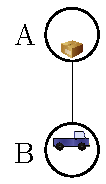
\includegraphics[scale=2]{pdfs/one-truck-one-package.pdf}}
  \raisebox{-0.5\height}{
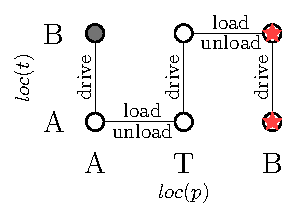
\includegraphics[scale=2]{pdfs/state-space-one-package.pdf}}
  \hspace*{1in}
  \raisebox{-0.5\height}{
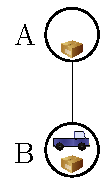
\includegraphics[scale=2]{pdfs/one-truck-two-packages.pdf}}
  \raisebox{-0.5\height}{
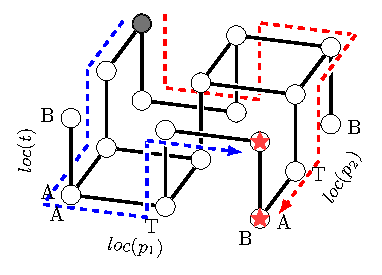
\includegraphics[scale=2]{pdfs/state-space-two-packages.pdf}}
\end{minipage}

\begin{itemize}
\item Optimal planning is to find a plan with the minimal cost.
\item Challenge: \embl{"state explosion problem"}

\end{itemize}
\end{myblock}


\begin{myblock}{Planning as Heuristic Search}
\Large
\begin{itemize}
\item Heuristics: estimations of shortest distance from state to goal
\item Heuristic Search:
\end{itemize}

\begin{minipage}{\textwidth}
  \centering
  \raisebox{-0.5\height}{
\includegraphics[scale=2.5]{pdfs/heuristic-search/{heuristic-search.tikz.preview}.pdf}}
  \raisebox{-0.5\height}{\includegraphics[scale=2.5]{pdfs/heuristic-search/{expanded.tikz.preview}.pdf}}
  \hspace*{0.3in}
  {\LARGE ...}
  \hspace*{0.3in}
  \raisebox{-0.5\height}{\includegraphics[scale=2.5]{pdfs/heuristic-search/{reached.tikz.preview}.pdf}}
\end{minipage}

\begin{itemize}
\item A* with \embl{admissible heuristics} $\rightarrow$ optimal planning
\end{itemize}

\end{myblock}


\begin{myblock}{Abstraction Heuristic}
\Large
\begin{itemize}
\item Abstraction is a mapping from the original state space to an abstract (and much smaller) one.
\item The distances of abstract states to the nearest abstract goal states are used as heuristic values
\end{itemize}

\begin{minipage}{\textwidth}
  \centering
  \raisebox{-0.5\height}{\includegraphics[scale=2.5]{pdfs/abstraction/{abstraction}.pdf}}
  \hspace*{0.5in}
  \raisebox{-0.5\height}{\includegraphics[scale=2.5]{pdfs/abstraction/{arrows}.pdf}}
  \hspace*{0.5in}
  \raisebox{-0.5\height}{\includegraphics[scale=2.5]{pdfs/abstraction/{abstract-space}.pdf}}
\end{minipage}

\begin{itemize}
\item Projection: consider some variables and ignore all others
\end{itemize}

\hspace*{-0.8in}
\begin{minipage}{\textwidth}
  \centering
  \raisebox{-0.5\height}{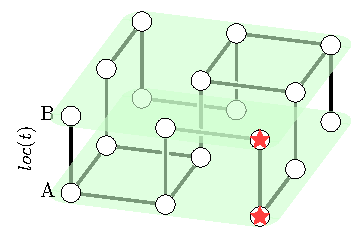
\includegraphics[scale=2.5]{pdfs/abstraction/ignore-packages.pdf}}
  \hspace*{0.1in}
  \raisebox{-0.5\height}{\includegraphics[scale=2.5]{pdfs/abstraction/{ignore-packages-arrow}.pdf}}
  \hspace*{0.5in}
  \raisebox{-0.5\height}{\includegraphics[scale=2.5]{pdfs/abstraction/{ignore-packages-abstract-space}.pdf}}
\end{minipage}

\begin{minipage}{\textwidth}
  \centering
  \raisebox{-0.5\height}{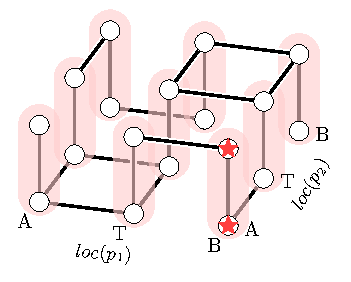
\includegraphics[scale=2.5]{pdfs/abstraction/ignore-truck.pdf}}
  \raisebox{-0.5\height}{\includegraphics[scale=2.5]{pdfs/abstraction/{ignore-truck-arrow}.pdf}}
  \raisebox{-0.5\height}{\includegraphics[scale=2.5]{pdfs/abstraction/{ignore-truck-abstract-space}.pdf}}
\end{minipage}

\end{myblock}
